\documentclass{lab}

\renewcommand{\AA}{\ensuremath{\mathring{A}}}

\begin{document}

\labtitle{4.1.3}{Рефрактометр Аббе}{7~марта~2019~г.}{14~марта~2019~г.}

\section*{Постановка эксперимента}

\begin{quote}
	\textbf{{\normalsize Цель работы: }}
	познакомится с методом измерения показателей преломления твёрдых и жидких сред в монохроматическом свете.
\end{quote}

\begin{quote}
	\textbf{{\normalsize Оборудование: }}
	технический рефрактометр Аббе; осветитель; набор стеклянных образцов;
	жидкости с неизвестными показателями преломления (глицерин, этиловый спирт);
	монобромнафталин; дистиллированная вода.
\end{quote}

\subsection*{Схема установки}

\begin{figure}[H]
	\centering
	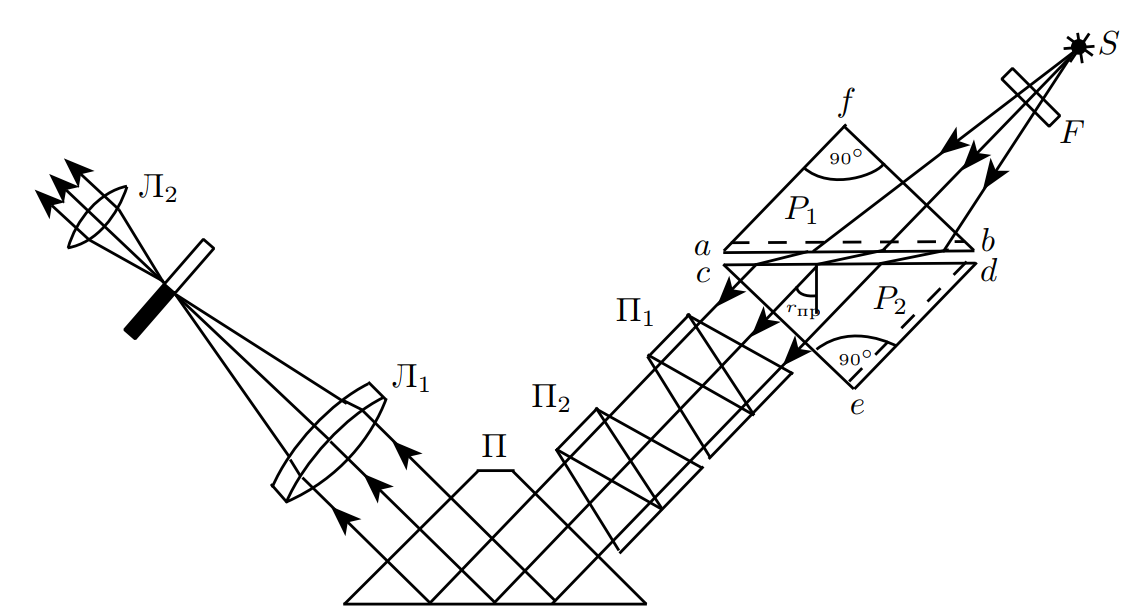
\includegraphics[width = \textwidth]{scheme_1}
	\caption{Ход лучей в рефрактометре при измерении показателя преломления жидкости методом скользящего луча}
	\label{scheme_1}
\end{figure}

\begin{figure}[H]
	\centering
	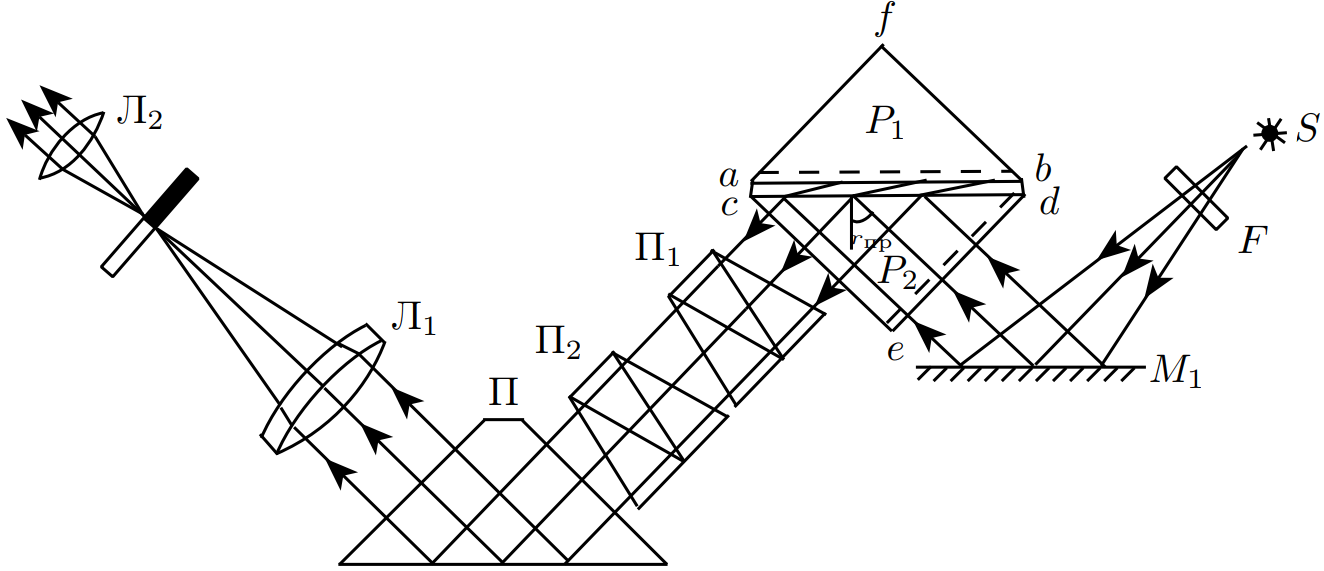
\includegraphics[width = \textwidth]{scheme_2}
	\caption{Ход лучей в рефрактометре при измерении показателя преломления жидкости методом полного внутреннего отражения}
	\label{scheme_2}
\end{figure}

\subsection*{Выполнение работы}

\begin{enumerate}
\item
Проделаем серию контрольных измерений показателя преломления дистиллированной воды:
\begin{table}[H]
	\centering
	\begin{tabular}{|c|cccccccc|}
		\hline
		n &1.3334 &1.331. &1.3325 &1.3331 &1.3320 &1.3335 &1.3329 &1.3330 \\\hline
	\end{tabular}
	\caption{Показатель преломления дистиллированной воды}
	\label{tab_1}
\end{table}

Погрешности измерений:
\begin{equation}
\begin{aligned}
&\sigma_{сист} = 10^{-4}\\
&\sigma_{случ}^2 = \dfrac{1}{\sqrt{N}} \cdot \sum_{i = 1}^{N} \left( x_i^2 - \langle x \rangle^2 \right) \approx 1.5 \cdot 10^{-4}
\end{aligned}
\end{equation}

Полученное значение $ n = (1.3327 \pm 0.0002) $ довольно точно совпадает с табличным значением $ n_0 = 1.33291 $.

\item
Измерим показатель преломления света двух стеклянных образцов, используя как метод скользящего луча, так и метод полного внутреннего отражения:
\begin{table}[H]
	\centering
	\begin{tabular}{|cc|cc|}
		\hline
		\multicolumn{2}{|c|}{1 образец} & \multicolumn{2}{c|}{2 образец} \\ \hline
		СЛ & ПВО & СЛ & ПВО \\
		1.5151 & 1.5160 & 1.5201 & 1.5185 \\
		1.5163 & 1.5201 & 1.5211 & 1.5169 \\
		1.5098 & 1.5146 & 1.5104 & 1.5181 \\
		1.5154 & 1.5158 & 1.5159 & 1.5099 \\
		1.5234 & 1.5261 & 1.5178 & 1.5174 \\ \hline
		\multicolumn{2}{|c|}{$ n = (1.5173 \pm 0.0002) $} & \multicolumn{2}{c|}{$ n = (1.5166 \pm 0.0002) $} \\ \hline
	\end{tabular}
	\caption{Показатель преломления дистиллированной воды}
	\label{tab_2}
\end{table}

\item
Аналогичным образом измерим показатели преломления глицерина и этилового спирта:
\begin{table}[H]
	\centering
	\begin{tabular}{|cc|cc|}
		\hline
		\multicolumn{2}{|c|}{Глицерин} & \multicolumn{2}{c|}{Этиловый спирт} \\ \hline
		СЛ & ПВО & СЛ & ПВО \\
		1.4694 & 1.4821 & 1.3620 & 1.3629 \\
		1.4810 & 1.4736 & 1.3614 & 1.3615 \\
		1.4792 & 1.4852 & 1.3634 & 1.3625 \\
		1.4823 & 1.4762 & 1.3625 & 1.3631 \\
		1.4831 & 1.4805 & 1.3641 & 1.3617 \\ \hline
		\multicolumn{2}{|c|}{$ n = (1.4793 \pm 0.0002) $} & \multicolumn{2}{c|}{$ n = (1.3625 \pm 0.0002) $} \\ \hline
	\end{tabular}
	\caption{Показатель преломления для разных веществ}
	\label{tab_3}
\end{table}

\item
По полученным экспериментальным данным вычислим молекулярные рефракции и поляризуемость молекул заданных жидкостей по формулам:
\begin{equation}
R = \dfrac{M}{\rho} \dfrac{n^2 - 1}{n^2 + 2} = \dfrac{1}{3} N_A \cdot \alpha \then \alpha = \dfrac{3R}{N_A}
\end{equation}
\begin{table}[H]
	\centering
	\begin{tabular}{|c|c|c|c|c|c|}
		\hline
		Вещество & $ n $ & $ \rho, ~ г/см^3 $ & $ M, ~ г/моль $ & R & $ \alpha, ~ 10^{-30} ~ м^3 $ \\ \hline
		Дист. вода & 1.3327 & 1 & 18 & 3.699 & 18.4 \\
		Глицерин & 1.4793 & 1.26 & 92.1 & 20.738 & 103.3 \\
		Этиловый спирт & 1.3625 & 0.789 & 46 & 12.947 & 64.5 \\ \hline
	\end{tabular}
	\caption{Молекулярная рефракция и поляризуемость молекул для разных веществ}
	\label{tab_4}
\end{table}

\item
Полагая рефракцию аддитивной, найдем атомные рефракции углерода, водорода и кислорода, полагая рефракции дистиллированной воды, глицерина и этилового спирта известными.
\begin{equation}
\begin{cases}
&R_{H_2O} = 2R_{H} + R_{O}\\
&R_{C_3H_8O_3} = 3R_{C} + 8R_{H} + 3R_{O}\\
&R_{C_2H_5OH} = 2R_{C} + 5R_{H} + R_{H} + R_{O}
\end{cases}
\then
\begin{cases}
&R_C = 2.508\\
&R_H = 1.057\\
&R_O = 1.583
\end{cases}
\end{equation}

\item
Полагая рефракции аддитивными, найдем рефракцию и показатель преломления метилового спирта:
\begin{equation}
\begin{aligned}
&R_{CH_4O} = R_C + 4R_H + R_O = 8.319\\
&R = \dfrac{M}{\rho}\dfrac{n^2 - 1}{n^2 + 2} \then n^2 = \dfrac{2R \rho + M}{M - R \rho}\\
&M = 32~г/моль, ~~~~~ \rho = 0.793~г/см^3 \then n = 1.3338\\
&Табличное ~ значение \then n_0 = 1.331
\end{aligned}
\end{equation}

Результаты подтверждают аддитивность рефракции.

\item
Аналогично проведем рассчет показателя преломления для льда и алмаза:
\begin{equation}
\begin{cases}
&n_{льда} = 1.3021\\
&n_{алмаза} = 3.0287
\end{cases}
~~~~~~~ Табличные значения \then
\begin{cases}
&n_{льда} = 1.31\\
&n_{алмаза} = 2.42
\end{cases}
\end{equation}

\end{enumerate}

\subsection*{Итоги}

Было проведено знакомство с устройством рефрактометра Аббе, были измерены коэффициенты преломления различными методами: методом скользящего луча и методом полного внутреннего отражения.\\

Познакомились с формулой Лоренц-Лоренца, убедились в аддитивности атомных и молекулярных рефракций для различных веществ.

\end{document}